\documentclass[10pt]{article}
\usepackage[polish]{babel}
\usepackage[utf8]{inputenc}
\usepackage[T1]{fontenc}
\usepackage{amsmath}
\usepackage{amsfonts}
\usepackage{amssymb}
\usepackage[version=4]{mhchem}
\usepackage{stmaryrd}
\usepackage{graphicx}
\usepackage[export]{adjustbox}
\graphicspath{ {./images/} }

\title{LIGA MATEMATYCZNA im. Zdzisława Matuskiego \\
 PAŹDZIERNIK 2015 \\
 GIMNAZJUM }

\author{}
\date{}


\begin{document}
\maketitle
\section*{ZADANIE 1.}
Wykaż, że liczba \(6^{100}-2 \cdot 6^{99}+10 \cdot 6^{98}\) jest podzielna przez 17 .

\section*{ZADANIE 2.}
W półokrąg o promieniu 5 wpisano dwa kwadraty, jak na rysunku. Oblicz sumę pól tych kwadratów.\\
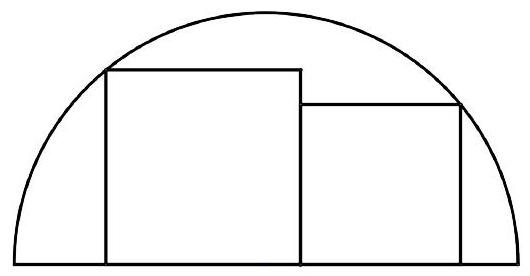
\includegraphics[max width=\textwidth, center]{2024_11_21_6cb928c4a60329347530g-1}

\section*{ZADANIE 3.}
Czy istnieją takie liczby naturalne \(m, n\), aby w wyniku mnożenia ich sumy przez ich iloczyn otrzymać liczbę 20162015?

\section*{ZADANIE 4.}
Rozważmy 1001 liczb: \(1,1+2,1+2+3,1+2+3+4, \ldots, 1+2+3+\ldots+1000,1+2+3+\ldots+1001\). Ile jest wśród nich liczb parzystych?

\section*{ZADANIE 5.}
Przygotowując prezent dla Ani, Bartek włożył go do małego pudełka, to pudełko włożył do większego, a to do jeszcze większego, przy czym każde następne pudełko całkowicie mieściło poprzednie. Ustal, w jakiej kolejności brał pudełka, jeżeli wiadomo, że:

\begin{itemize}
  \item pudełko żółte jest prostopadłościanem o objętości \(12144 \mathrm{~cm}^{3}\) i jego jedna ściana ma wymiary 23 cm i 24 cm ;
  \item pudełko zielone jest sześcianem o objętości \(8000 \mathrm{~cm}^{3}\);
  \item pudełko różowe jest sześcianem o sumie długości wszystkich krawędzi równej 312 cm .
\end{itemize}

\end{document}